\documentclass[11pt,openany]{book}
% ============================================================
%  Snake, Learned by Playing Itself -- report preamble
%  (adapted from the 10-703 notes preamble: same palette, boxes and headings)
% ============================================================
\usepackage[T1]{fontenc}
\usepackage[utf8]{inputenc}
\usepackage{lmodern}
\usepackage{microtype}
\usepackage{amsmath,amssymb,amsthm,mathtools}
\usepackage{bm}
\usepackage{xcolor}
\usepackage{graphicx}
\usepackage{booktabs}
\usepackage{array}
\usepackage{enumitem}
\usepackage{etoolbox}
\usepackage{tikz}
\usepackage{pgfplots}
\pgfplotsset{compat=1.18}
\usepackage{caption}
\usepackage{listings}
\usepackage{multirow}
\usetikzlibrary{arrows.meta,positioning,calc,fit,backgrounds,decorations.pathreplacing,shapes.geometric,patterns}
\usepackage{framed}
\usepackage{titlesec}
\usepackage{fancyhdr}
\usepackage[hidelinks,colorlinks=true,linkcolor=cmured,citecolor=cmured,urlcolor=cmured]{hyperref}

% ---------- palette ----------
\definecolor{cmured}{HTML}{A6192E}
\definecolor{cmudark}{HTML}{6E1220}
\definecolor{inkblue}{HTML}{1F3A5F}
\definecolor{seagreen}{HTML}{1B6B5A}
\definecolor{amber}{HTML}{B8860B}
\definecolor{softgrey}{HTML}{F4F2F0}
\definecolor{rulegrey}{HTML}{CFC9C4}
\definecolor{boxcream}{HTML}{FDF6E3}
\definecolor{boxblue}{HTML}{EDF2F8}
\definecolor{boxgreen}{HTML}{EDF5F2}
\definecolor{boxred}{HTML}{FBEEF0}

% ---------- page ----------
\usepackage[margin=1.05in,top=1.15in,bottom=1.15in,headheight=15pt]{geometry}
\setlength{\parskip}{0.55em}
\setlength{\parindent}{0pt}
\renewcommand{\arraystretch}{1.25}

\pagestyle{fancy}
\fancyhf{}
\renewcommand{\headrulewidth}{0.4pt}
\renewcommand{\headrule}{\hbox to\headwidth{\color{rulegrey}\leaders\hrule height \headrulewidth\hfill}}
\fancyhead[L]{\footnotesize\color{cmudark}\scshape\nouppercase{\leftmark}}
\fancyhead[R]{\footnotesize\color{cmudark}\thepage}
\fancypagestyle{plain}{\fancyhf{}\renewcommand{\headrulewidth}{0pt}\fancyhead[R]{\footnotesize\color{cmudark}\thepage}}

% ---------- headings ----------
\titleformat{\chapter}[display]
  {\normalfont\huge\bfseries\color{cmured}}
  {\hfill\normalfont\sffamily\fontsize{58}{58}\selectfont\color{rulegrey}\thechapter}
  {-12pt}
  {\raggedright\color{cmudark}}
  [\vspace{4pt}{\color{cmured}\titlerule[1.4pt]}]
\titlespacing*{\chapter}{0pt}{-30pt}{26pt}

\titleformat{\section}
  {\normalfont\large\bfseries\color{cmured}}{\thesection}{0.7em}{}
\titleformat{\subsection}
  {\normalfont\normalsize\bfseries\color{cmudark}}{\thesubsection}{0.6em}{}
\titlespacing*{\section}{0pt}{1.5em}{0.5em}
\titlespacing*{\subsection}{0pt}{1.1em}{0.35em}

% ---------- boxes ----------
% page-breakable coloured callouts built on framed
\newlength{\cbarw}\setlength{\cbarw}{2.6pt}
\newenvironment{@cbox}[3]% #1 = background, #2 = bar colour, #3 = title text
{%
  \par\addvspace{9pt}%
  \def\FrameCommand{{\color{#2}\vrule width \cbarw}\hspace{0pt}\colorbox{#1}}%
  \MakeFramed{\advance\hsize-\width\FrameRestore}%
  \noindent\hspace{6pt}%
  \begin{minipage}{\dimexpr\linewidth-12pt\relax}%
  \vspace{3pt}%
  \ifstrempty{#3}{}{{\sffamily\bfseries\color{#2}#3\par\vspace{2pt}}}%
  \setlength{\parskip}{0.45em}%
}
{%
  \vspace{3pt}\end{minipage}\hspace{6pt}%
  \endMakeFramed\par\addvspace{9pt}%
}

\newenvironment{defbox}[1][]{\begin{@cbox}{boxblue}{inkblue}{#1}}{\end{@cbox}}
\newenvironment{keybox}[1][]{\begin{@cbox}{boxcream}{amber}{#1}}{\end{@cbox}}
\newenvironment{algbox}[1][]{\begin{@cbox}{boxgreen}{seagreen}{#1}}{\end{@cbox}}
\newenvironment{warnbox}[1][]{\begin{@cbox}{boxred}{cmured}{#1}}{\end{@cbox}}


% ---------- numbered results + two-way proof links ----------
\makeatletter
\@ifundefined{c@chapter}
  {\newcounter{resct}\renewcommand{\theresct}{\arabic{resct}}}
  {\newcounter{resct}[chapter]\renewcommand{\theresct}{\thechapter.\arabic{resct}}}
\makeatother

% \begin{namedresult}{key}{Kind}{Title} ... \end{namedresult}
\newenvironment{namedresult}[3]{%
  \refstepcounter{resct}%
  \begin{@cbox}{boxblue}{inkblue}{#2~\theresct\ \ #3}%
  \label{res:#1}%
}{\end{@cbox}}

% pointer placed inside a result when its proof lives elsewhere
\newcommand{\proofat}[1]{%
  \par\vspace{1pt}%
  {\footnotesize\color{seagreen}$\blacktriangleright$~\hyperref[pf:#1]{Proof on page~\pageref*{pf:#1}}}}

% \begin{proofof}{key}{Kind}{Title} ... \end{proofof}
\newenvironment{proofof}[3]{%
  \begin{@cbox}{boxgreen}{seagreen}{Proof of #2~\ref*{res:#1} \ #3}%
  \label{pf:#1}%
  {\footnotesize\color{inkblue}$\blacktriangleleft$~\hyperref[res:#1]{Statement on page~\pageref*{res:#1}}}%
  \par\vspace{2pt}%
}{\end{@cbox}}

% restatement block shown at a remote proof site
\newcommand{\restated}[1]{%
  \par{\small\itshape\color{cmudark}Restated.\ }\ignorespaces #1\par\vspace{2pt}}

% proof-index row
\newcommand{\pidx}[2]{%
  \hyperref[res:#1]{#2} & \pageref*{res:#1} & \hyperref[pf:#1]{\pageref*{pf:#1}}\\}

% cross-reference helper used in prose
\newcommand{\seeres}[2]{\hyperref[res:#1]{#2~\ref*{res:#1}}}

% ---------- notation macros ----------
\newcommand{\Sspace}{\mathcal{S}}
\newcommand{\Aspace}{\mathcal{A}}
\newcommand{\Dbuf}{\mathcal{D}}
\newcommand{\E}{\mathbb{E}}
\newcommand{\Prob}{\mathbb{P}}
\newcommand{\Real}{\mathbb{R}}
\newcommand{\Hent}{\mathcal{H}}
\newcommand{\KL}{D_{\mathrm{KL}}}
\newcommand{\TV}{D_{\mathrm{TV}}}
\newcommand{\Adv}{A}
\newcommand{\Qs}{Q}
\newcommand{\Vs}{V}
\newcommand{\pol}{\pi}
\newcommand{\beh}{\mu}
\newcommand{\dpi}{d^{\pi}}
\newcommand{\dmu}{d^{\mu}}
\newcommand{\clip}{\operatorname{clip}}
\newcommand{\Tr}{\mathcal{T}}
\newcommand{\defeq}{\vcentcolon=}
\newcommand{\st}{\;\middle|\;}

% tighter lists
\setlist[itemize]{leftmargin=1.25em,itemsep=2pt,topsep=3pt,parsep=0pt}
\setlist[enumerate]{leftmargin=1.5em,itemsep=2pt,topsep=3pt,parsep=0pt}

% tikz styles
\tikzset{
  node box/.style={draw=cmured,line width=0.8pt,rounded corners=2pt,fill=white,
                   inner sep=5pt,font=\small,align=center},
  node fill/.style={draw=cmured,line width=0.8pt,rounded corners=2pt,fill=cmured,
                   text=white,inner sep=5pt,font=\small\bfseries,align=center},
  node soft/.style={draw=rulegrey,line width=0.8pt,rounded corners=2pt,fill=softgrey,
                   inner sep=5pt,font=\small,align=center},
  flow/.style={-{Stealth[length=5pt]},line width=0.9pt,draw=cmudark},
  flowdash/.style={-{Stealth[length=5pt]},line width=0.9pt,draw=cmudark,dashed},
  lbl/.style={font=\scriptsize\itshape,inner sep=2pt},
}

% ---------- report additions ----------
\captionsetup{font=small,labelfont={sf,bf,color=cmudark},textfont={color=cmudark},
  labelsep=period,skip=6pt}

\definecolor{snakeorange}{HTML}{F59E0B}
\definecolor{snakeblue}{HTML}{38BDF8}
\definecolor{boardbg}{HTML}{0E1426}

\lstdefinestyle{report}{
  basicstyle=\ttfamily\small\color{cmudark},
  keywordstyle=\color{cmured}\bfseries,
  commentstyle=\color{seagreen}\itshape,
  stringstyle=\color{inkblue},
  backgroundcolor=\color{softgrey},
  frame=leftline, framerule=2.6pt, rulecolor=\color{rulegrey},
  xleftmargin=10pt, framexleftmargin=6pt, aboveskip=8pt, belowskip=8pt,
  columns=fullflexible, keepspaces=true, showstringspaces=false,
  breaklines=true, tabsize=4,
}
\lstset{style=report}

\pgfplotsset{
  reportaxis/.style={
    width=\linewidth, height=6.2cm,
    axis line style={rulegrey}, tick style={rulegrey},
    tick label style={font=\footnotesize,color=cmudark},
    label style={font=\small,color=cmudark},
    grid=major, major grid style={rulegrey!45},
    legend style={draw=none,fill=none,font=\footnotesize,text=cmudark},
    legend cell align=left,
    every axis plot/.append style={line width=1.15pt},
  },
}

\newcommand{\code}[1]{\texttt{\color{cmudark}#1}}
\newcommand{\pct}[1]{#1\%}


\title{Snake, Learned by Playing Itself}
\author{Alex Kozik}
\date{October 2026}

\begin{document}

% ---------------- title page ----------------
\begin{titlepage}
\thispagestyle{empty}
\begin{tikzpicture}[remember picture, overlay]
  \fill[cmured] ([xshift=0cm,yshift=-3.2cm]current page.north west)
    rectangle ([xshift=0cm,yshift=-3.35cm]current page.north east);
\end{tikzpicture}
\vspace*{3.2cm}

{\raggedright
{\fontsize{15}{18}\selectfont\sffamily\color{cmudark} Technical report\par}
\vspace{0.8cm}
{\fontsize{44}{48}\selectfont\bfseries\color{cmured} Snake, Learned\\[4pt] by Playing Itself\par}
\vspace{0.7cm}
{\fontsize{16}{20}\selectfont\color{cmudark}\itshape Self-play reinforcement learning for\\[2pt]
  multi-agent Battlesnake, from simulator to browser\par}
\vspace{1.1cm}
{\color{rulegrey}\rule{0.42\linewidth}{1pt}}
\vspace{0.7cm}

{\normalsize\color{cmudark}
\begin{tabular}{@{}r@{\hspace{1.2em}}l@{}}
\textbf{1} & Introduction\\
\textbf{2} & The Game\\
\textbf{3} & A Batched Simulator\\
\textbf{4} & Verifying the Simulator\\
\textbf{5} & Observations, Rewards and Masks\\
\textbf{6} & Scripted Opponents and Measurement\\
\textbf{7} & Learning by Self-Play\\
\textbf{8} & Results: The Duel\\
\textbf{9} & Results: The Arena\\
\textbf{10} & Into the Browser\\
\textbf{11} & Limitations and Next Steps\\
\end{tabular}\par}
\vfill
{\footnotesize\color{cmudark} October 2026\qquad$\cdot$\qquad Alex Kozik\qquad$\cdot$\qquad
  \href{https://github.com/LambdaAK/SnakeDQN}{github.com/LambdaAK/SnakeDQN}\par}
}
\end{titlepage}

% ---------------- at a glance ----------------
\chapter*{At a glance}
\addcontentsline{toc}{chapter}{At a glance}
\markboth{At a glance}{}

This report documents a complete reinforcement-learning system for
\emph{Battlesnake}, the simultaneous-move, multi-player variant of Snake. Two neural
networks were trained from scratch by self-play, with no human data and no hand-written
features, and both now run live in a web page. The report covers every layer: the game
rules and their batched implementation, how that implementation was verified, the
learning algorithm, the experiments, and the browser port.

\begin{keybox}[Headline results]
\textbf{Duel} (two snakes, $11\times11$). After 2.5 hours of self-play on a laptop
(33.6M game turns), the network wins \textbf{91.4\%} of 1{,}000 games against the
strongest hand-written bot (95\% CI 89.5--93.0), and \textbf{90.2\%} against a
food-greedy bot. For comparison, the strongest bot beats the greedy one only 74.0\% of the
time.

\textbf{Arena} (six snakes, $19\times19$). A second network that sees only a
$17\times17$ window around its own head wins \textbf{44.7\%} of 300 games played as one
snake against \emph{five} flood-fill bots. An even contest would win
$1/6 \approx 16.7\%$.
\end{keybox}

\begin{center}
\begin{tabular}{@{}lrr@{}}
\toprule
\textbf{Component} & \textbf{Figure} & \textbf{Where}\\
\midrule
Simulator throughput & 214{,}000 turns/s & Chapter~\ref{ch:sim}\\
Automated tests & 106 & Chapter~\ref{ch:verify}\\
Duel network & 2.04M parameters, 8.2\,MB ONNX & Chapter~\ref{ch:learn}\\
Arena network & 2.43M parameters, 9.7\,MB ONNX & Chapter~\ref{ch:arena}\\
Duel win rate vs flood-fill bot & 91.4\% & Chapter~\ref{ch:duel}\\
Arena win rate vs $5\times$ flood-fill & 44.7\% & Chapter~\ref{ch:arena}\\
Training budget, each network & 2.5\,h, Apple M3 Max GPU & Chapter~\ref{ch:learn}\\
\bottomrule
\end{tabular}
\end{center}

\textbf{How to read this report.} Four kinds of box appear throughout, as in the
course notes this layout is borrowed from.

\noindent\begin{minipage}[t]{0.485\linewidth}
\begin{defbox}[Definition]
A formal object, rule or quantity.
\end{defbox}
\begin{algbox}[Algorithm]
A procedure, as implemented.
\end{algbox}
\end{minipage}\hfill
\begin{minipage}[t]{0.485\linewidth}
\begin{keybox}[Key idea]
The load-bearing decision or insight.
\end{keybox}
\begin{warnbox}[Watch out]
A subtlety, a bug found and fixed, or a caveat.
\end{warnbox}
\end{minipage}

\clearpage
\pagestyle{plain}
\tableofcontents
\clearpage
\pagestyle{fancy}

\chapter{Introduction}\label{ch:intro}

Snake is a game most people learn in an afternoon: steer, eat, grow, and do not run into
anything. Battlesnake turns it into a competitive, simultaneous-move game for several
players, where the board fills up with bodies and two heads meeting on the same cell
settle the matter by length. It is small enough to simulate millions of times an hour,
yet rich enough that good play needs planning: cutting opponents off, avoiding traps you
cannot see the bottom of, and knowing when to eat and when to fight.

This project builds, from the ground up, an agent that learns this game entirely by
playing against copies of itself, and puts the result in a web page where anyone can
watch it or play against it.

\section{Goals}

\begin{enumerate}
\item \textbf{A faithful, fast simulator.} Standard Battlesnake rules, batched so that
  thousands of games advance in one vectorised step, with correctness established by
  independent means rather than assumed.
\item \textbf{Learning without priors.} No human games, no hand-engineered features in the
  observation, and a reward that only says who won.
\item \textbf{Honest measurement.} Fixed scripted opponents, many games, confidence
  intervals, and checkpoint selection that does not leak into the reported numbers.
\item \textbf{A live demonstration.} The trained networks run client-side in a browser,
  on a port of the rules that is checked move-for-move against the original.
\end{enumerate}

\section{System overview}

\begin{center}
\begin{tikzpicture}[node distance=0.55cm and 0.9cm]
  \node[node fill, text width=2.6cm] (rules) {Rules\\\footnotesize batched NumPy};
  \node[node box, right=of rules, text width=2.6cm] (obs) {Observations\\\footnotesize egocentric planes};
  \node[node box, right=of obs, text width=2.6cm] (ppo) {PPO self-play\\\footnotesize PyTorch, MPS};
  \node[node fill, right=of ppo, text width=2.2cm] (onnx) {ONNX\\\footnotesize export};
  \node[node soft, below=0.9cm of rules, text width=2.6cm] (oracle) {Reference oracle\\\footnotesize pure Python};
  \node[node soft, below=0.9cm of obs, text width=2.6cm] (bots) {Scripted bots\\\footnotesize 5 baselines};
  \node[node soft, below=0.9cm of ppo, text width=2.6cm] (harness) {Match harness\\\footnotesize Wilson CIs};
  \node[node soft, below=0.9cm of onnx, text width=2.2cm] (js) {JS rules\\\footnotesize + web demo};
  \draw[flow] (rules) -- (obs);
  \draw[flow] (obs) -- (ppo);
  \draw[flow] (ppo) -- (onnx);
  \draw[flowdash] (oracle) -- node[lbl,left]{checks} (rules);
  \draw[flowdash] (bots) -- (harness);
  \draw[flowdash] (harness) -- node[lbl,right]{scores} (ppo);
  \draw[flow] (onnx) -- (js);
  \draw[flowdash] (rules.west) -- ++(-0.35,0) |- ($(js.south)+(0,-0.5)$)
    node[lbl,below,pos=0.75]{parity tests} -- (js.south);
\end{tikzpicture}
\end{center}

The work is organised in layers, each of which is tested against something independent
of itself:

\begin{itemize}
\item the \textbf{rules} (Chapter~\ref{ch:sim}) against a slow reference implementation
  and against themselves run one game at a time (Chapter~\ref{ch:verify});
\item the \textbf{observations and rewards} (Chapter~\ref{ch:obs}) against hand-built
  positions;
\item the \textbf{agents} against five scripted bots through a common evaluation
  harness (Chapter~\ref{ch:baselines});
\item the \textbf{browser port} (Chapter~\ref{ch:browser}) against Python-generated
  trajectories.
\end{itemize}

\section{Contributions}

\begin{keybox}[What this report shows]
\begin{enumerate}
\item A batched Battlesnake engine in pure NumPy reaching 214{,}000 game turns per second
  on a laptop CPU, verified exactly against an independent oracle.
\item A duel network that beats the best hand-written heuristic in 91\% of games after
  2.5 hours of training, learned from a $\pm1$ win signal.
\item A head-centred \emph{window} observation that decouples the network from board size
  and player count, enabling a six-snake arena agent that wins nearly three times its fair
  share against a table of flood-fill bots.
\item A browser deployment with continuous rendering of a turn-based game, and a
  JavaScript rules port verified against the Python engine.
\end{enumerate}
\end{keybox}

\section{A note on history}

The repository began as a single-snake Deep Q-Network with a hand-crafted 33-number
state: danger flags, A* path quality, dead-end lookahead. That design leaned on features
that already encoded much of the answer, ran a path search four times per step, and
could not express a second player. The rebuild described here discards those features,
replaces the single-player game with the full multi-player rules, and moves from DQN to
PPO. Comparing value-based and policy-gradient methods on the new environment is left as
future work (Chapter~\ref{ch:limits}).

\chapter{The Game}\label{ch:game}

\begin{center}

\includegraphics[width=0.46\linewidth]{figures/duel_board.png}
\captionof{figure}{A duel at turn 45, both seats played by the trained network. Heads
are the larger discs; red dots are food.}
\label{fig:duel-board}
\end{center}

\section{The board and the snakes}

\begin{defbox}[Game state]
A game is played on a $B\times B$ grid of cells $(r,c)$, row $0$ at the top, with
$B\ge 7$ ($B=11$ by default). It has $S\in\{1,\dots,8\}$ snakes. Snake $k$ has
\begin{itemize}
\item a \emph{body} $\bigl(x^k_0, x^k_1, \dots, x^k_{L_k-1}\bigr)$, a list of cells with the head
  $x^k_0$ first. Cells may repeat; this matters, see below.
\item a \emph{length} $L_k$, the number of entries in the body;
\item a \emph{health} $h_k \in \{0,\dots,h_{\max}\}$ with $h_{\max}=100$;
\item an \emph{alive} flag.
\end{itemize}
The board also holds a set of food cells $F$, a turn counter, and the game's
\emph{minimum food} $f_{\min}$, which is $1$ in standard play.
\end{defbox}

\textbf{Actions.} Every turn each living snake chooses one of four absolute directions,
$a\in\{\uparrow,\downarrow,\leftarrow,\rightarrow\}$, encoded $0$--$3$. All snakes move
\emph{simultaneously}; nobody sees the others' choices before committing. Reversing onto
your own neck is legal but fatal, exactly as in the official game.

\section{One turn}

\begin{algbox}[Turn order (Battlesnake standard)]
Given every snake's action:
\begin{enumerate}
\item \textbf{Move.} Each living snake's body becomes $\bigl(x_0 + \delta(a),\ x_0,\ \dots,\ x_{L-2}\bigr)$:
  a new head is added and the last segment drops off.
\item \textbf{Health.} Every moving snake loses one health point.
\item \textbf{Feed.} A snake whose new head is on food resets its health to $h_{\max}$
  and \emph{duplicates its last segment}, so its length grows by one. The food is removed
  after all snakes have fed, so two heads on one food both eat.
\item \textbf{Spawn food.} If $|F| < f_{\min}$, or with probability $15\%$ otherwise, one
  food appears on a uniformly random free cell.
\item \textbf{Eliminate.} First remove every snake that starved ($h\le 0$) or left the
  board. Then, simultaneously among the rest, a snake is eliminated if its head lies on
  any body segment other than a head (its own included), or if it meets another head
  whose snake is \emph{at least as long}.
\item \textbf{End.} With $S>1$ the game ends when at most one snake is alive; the
  survivor, if any, wins. A single snake's game ends when it dies.
\end{enumerate}
\end{algbox}

\begin{warnbox}[Growth is a duplicated tail, not an extra head]
When a snake eats, its tail stays put \emph{on the next turn}, because the duplicated
segment is what drops off. Two consequences follow, and both are easy to get wrong:
\begin{itemize}
\item moving into a cell that an opponent's tail is vacating is \emph{safe}, unless that
  opponent ate last turn, in which case the tail does not move and the move is fatal;
\item a snake's length counts the duplicate. A snake that fills all $64$ cells of an
  $8\times8$ board by eating the food spawned into its own vacated tail cell ends with
  length $65$, not $64$. This was caught by a test (Chapter~\ref{ch:baselines}).
\end{itemize}
\end{warnbox}

\section{Head-to-head collisions}

The head-to-head rule is what makes the game strategic rather than a race to eat. Let
$P_k$ be the cell snake $k$ moves into. Snake $k$ is eliminated by a head-to-head if
\[
  \exists\, j\ne k:\quad P_j = P_k \ \text{ and }\ L_j \ge L_k .
\]
Equal lengths eliminate \emph{both} snakes. Being longer therefore makes a snake a
threat to every neighbouring head, and this is exactly what one of the observation
planes encodes (Chapter~\ref{ch:obs}).

\section{Setup}

\begin{defbox}[Start positions and initial food]
Let $a=1$, $m=\lfloor B/2\rfloor$, $z=B-2$. The eight start cells are the four
\emph{corners} $\{(a,a),(a,z),(z,a),(z,z)\}$ and the four \emph{edge midpoints}
$\{(a,m),(m,a),(m,z),(z,m)\}$. Each game picks one group with probability $\tfrac12$ and
fills it first, in random order, so with $S\le4$ snakes all start equidistant from the
centre. Every snake starts with length $3$, all three segments stacked on its start cell.

Food is placed on the centre cell, and for each snake on one of its four diagonal
neighbours, chosen uniformly among those that are not a board corner and are not
strictly closer to the centre than the snake itself.
\end{defbox}

\section{As a Markov game}

For learning, the game is a stochastic game with $S$ players. The state is
the full board; the transition is the turn order above, whose only randomness is food
spawning; and each player's reward is
\[
  R_k \;=\;
  \begin{cases}
    +1 & \text{if } k \text{ is the last snake alive,}\\
    -1 & \text{on the turn } k \text{ is eliminated, unless every remaining snake falls on that turn,}\\
    \hphantom{+}0 & \text{otherwise.}
  \end{cases}
\]
A turn on which the last snakes all fall together is a \emph{draw}, worth $0$ to each of
them. Each player observes the board from its own point of view (Chapter~\ref{ch:obs}).
Because every seat runs the same rules and sees an egocentric view, a single policy
network can play every seat at once, which is what self-play exploits.

\chapter{A Batched Simulator}\label{ch:sim}

Reinforcement learning is hungry for experience: the duel network in this report saw
36 million game turns. A Python loop over games would make that a week; the simulator
instead advances $N$ games in a single vectorised step, with no Python loop over games
anywhere on the training path.

\section{State as arrays}

\begin{defbox}[Batched game state]
All games in a batch share the board size $B$ and snake count $S$. The state is a
handful of NumPy arrays indexed \code{[env, snake, ...]}:
\begin{center}
\begin{tabular}{@{}llp{0.5\linewidth}@{}}
\toprule
\textbf{Field} & \textbf{Shape, dtype} & \textbf{Meaning}\\
\midrule
\code{body}   & $(N,S,B^2{+}1,2)$, int16 & segment cells, head at index 0\\
\code{length} & $(N,S)$, int16 & number of valid segments\\
\code{health} & $(N,S)$, int16 & health points\\
\code{alive}  & $(N,S)$, bool  & snake is in play\\
\code{food}   & $(N,B,B)$, bool & food cells\\
\code{turn}   & $(N)$, int32 & turns played\\
\code{over}   & $(N)$, bool & game finished, awaiting reset\\
\bottomrule
\end{tabular}
\end{center}
Segments past \code{length} are garbage and never read. The extra slot in
$B^2{+}1$ holds the duplicated tail of a snake that has filled the board.
\end{defbox}

\begin{keybox}[Why a fixed-capacity body array]
Storing every body in a padded array of capacity $B^2{+}1$ turns ``move every snake''
into one slice assignment, \code{body[m, 1:L] = body[m, 0:L-1]}, over the boolean mask
$m$ of moving snakes, with $L$ the longest current length plus one. Short games pay
only for their actual length, and no per-snake Python list ever exists.
\end{keybox}

\section{The step, vectorised}

Each stage of the turn order (Chapter~\ref{ch:game}) maps to a few array operations.

\begin{algbox}[\code{step\_games(state, actions, spawn\_u)}]
\begin{enumerate}
\item \textbf{Validate} that \code{actions} is an integer array of shape $(N,S)$ with
  values in $0..3$; anything else raises, rather than silently wrapping.
\item \textbf{Move} the masked snakes by slicing, write the new heads, and decrement
  health.
\item \textbf{Feed} by looking up \code{food[env, row, col]} at every new head (clipped
  for off-board heads, which are masked out). Eaters duplicate their tail with one fancy
  assignment, reset health, and clear the food.
\item \textbf{Spawn} at most one food per game, driven by the externally supplied
  uniforms \code{spawn\_u} (next section).
\item \textbf{Eliminate}: compute survivors of starvation and walls; build an occupancy
  count of their non-head segments; look up each head in it; resolve head-to-heads with an
  $S\times S$ comparison of head cells and lengths.
\item \textbf{Finish}: advance turns, flag finished games, and report per-snake
  \code{ate}, \code{died} and \code{alive\_before}, plus per-game \code{game\_over} and
  \code{winner}.
\end{enumerate}
\end{algbox}

\subsection{Occupancy by \code{bincount}}

Several stages ask the same question: how many segments of which snakes sit on each cell?
Flattening every cell of every game to one index
\[
  \iota(n, r, c) = (n\cdot B + r)\cdot B + c,
\]
the answer for any mask of snakes and range of segment indices is a single
\code{np.bincount} over the valid segments, reshaped to $(N, B^2)$. Body collisions use
segments $1..L{-}1$ of survivors; the action mask uses segments $0..L{-}2$ of living
snakes, since tails move away; food spawning uses all segments.

\subsection{Head-to-head without loops}

With $\text{cell}_k$ the flattened new head of snake $k$ and $\text{surv}_k$ its survivor
flag, snake $k$ loses a head-to-head if
\[
  \bigvee_{j\ne k}\ \bigl[\text{cell}_j = \text{cell}_k\bigr]\wedge
  \text{surv}_j \wedge \text{surv}_k \wedge \bigl[L_j \ge L_k\bigr],
\]
an $(N,S,S)$ boolean tensor reduced over $j$. With $S\le 8$ this is cheaper than any
alternative.

\section{Randomness you can replay}

\begin{keybox}[Injected uniforms]
The step function takes its randomness as an argument: two uniforms per game,
$u_0,u_1\sim\mathcal{U}[0,1)$. A food spawns if $|F|<f_{\min}$ or $u_0<0.15$, on the
$\lfloor u_1\cdot n_{\text{free}}\rfloor$-th free cell in row-major order. Given the same
uniforms, any implementation must place food on exactly the same cell. This is what lets
the batched engine, a slow reference engine, and a JavaScript port be compared
\emph{exactly}, step for step (Chapter~\ref{ch:verify}).
\end{keybox}

Choosing the $k$-th free cell is itself vectorised: with \code{free} an $(n,B^2)$
boolean array, the cell is \code{argmax(cumsum(free, axis=1) > k)}.

\section{The environment wrapper}

\code{SnakeEnv} wraps the rules in the usual interface. Its constructor takes the number
of games, the number of snakes, the board size, a reward name, the maximum health, a seed
and the minimum food:
\begin{lstlisting}[language=Python]
env = SnakeEnv(num_envs=1024, num_snakes=2)        # 11x11 Battlesnake
obs, info = env.reset()                            # obs: (1024, 2, 8, 11, 11)
obs, rewards, dones, info = env.step(actions)      # actions: (1024, 2) in {0,1,2,3}
\end{lstlisting}

Finished games \textbf{reset automatically} inside \code{step}. The returned \code{obs}
is the first frame of the new game, while \code{info} carries \code{final\_obs},
\code{final\_length}, \code{final\_turn}, \code{winner} and \code{game\_over} for the
game that just ended. It also exposes the \code{action\_mask} and the \code{active}
mask, which Chapter~\ref{ch:obs} explains.

\section{Performance}

\begin{center}
\begin{tikzpicture}
\begin{axis}[reportaxis, height=4.6cm, width=0.72\linewidth, xbar, xmin=150, xmax=230,
  symbolic y coords={Initial version, + spawn occupancy mask, + preallocated observations},
  ytick=data, y dir=reverse, bar width=11pt, enlarge y limits=0.28,
  xlabel={thousand game turns per second (1{,}024 games, 2 snakes)},
  nodes near coords, nodes near coords style={font=\footnotesize,color=cmudark},
  grid=none]
\addplot[fill=cmured!80, draw=none] coordinates
  {(198,Initial version) (206,+ spawn occupancy mask) (214,+ preallocated observations)};
\addplot[draw=cmudark, dashed, line width=0.8pt, sharp plot, nodes near coords={}] coordinates
  {(200,Initial version) (200,+ preallocated observations)};
\end{axis}
\end{tikzpicture}
\captionof{figure}{Simulator throughput on an Apple M3 Max CPU (medians of repeated runs;
the machine varies by about 5\% between runs). The dashed line is the 200{,}000 target.}
\label{fig:throughput}
\end{center}

The target was 200{,}000 turns per second. Profiling the first version showed time split
between building observations (\code{np.stack}, 18\%), occupancy counting (17\%) and
per-snake layer drawing (14\%). Two changes cleared the target without touching
behaviour:
\begin{itemize}
\item \textbf{Spawn occupancy only where needed.} About 15\% of games spawn food on a
  given turn; counting occupancy only for those games removes most of that work.
\item \textbf{Preallocated observations.} Writing each channel into one preallocated
  array instead of stacking eight temporaries.
\end{itemize}
A direct comparison of the old and new code over 300 turns of 256 games, in four
configurations up to eight snakes on $19\times19$, produced identical states and
observations at every step.

\chapter{Verifying the Simulator}\label{ch:verify}

A fast simulator with a subtle bug is worse than a slow correct one: the agent will
learn to exploit the bug, and every result built on top inherits it. The engine is
therefore checked four independent ways, and all 106 automated tests run on every push.

\begin{center}
\begin{tikzpicture}[node distance=0.5cm and 0.6cm]
  \node[node fill, text width=2.8cm] (eng) {Batched engine\\\footnotesize NumPy};
  \node[node box, above left=0.5cm and 0.4cm of eng, text width=2.8cm] (unit) {Rule tests\\\footnotesize hand-built boards};
  \node[node box, above right=0.5cm and 0.4cm of eng, text width=2.8cm] (oracle) {Reference oracle\\\footnotesize plain Python lists};
  \node[node box, below left=0.5cm and 0.4cm of eng, text width=2.8cm] (batch) {Batch consistency\\\footnotesize $N$ games vs 1 game};
  \node[node box, below right=0.5cm and 0.4cm of eng, text width=2.8cm] (js) {JavaScript parity\\\footnotesize browser port};
  \foreach \n in {unit,oracle,batch,js} \draw[flowdash] (\n) -- (eng);
\end{tikzpicture}
\end{center}

\section{Rule tests}

Each rule has a test on a hand-built board: walls, self-collision, neck reversal, moving
into a vacating tail (safe), moving into a tail that just ate (fatal), eating, starving,
eating on the last health point (survives), head-to-head with longer, shorter and equal
opponents, collisions with another snake's body and its vacating tail, actions for dead
snakes and finished games (ignored), forced and random food spawns, a completely full
board (no spawn, no crash), and malformed actions (rejected).

\section{An independent reference implementation}

\begin{defbox}[Reference oracle]
A second implementation of the rules for a single game, written for readability:
bodies are Python lists, collisions use a \code{Counter}, free cells are enumerated in
row-major order. It shares no code with the batched engine.
\end{defbox}

\begin{algbox}[Oracle comparison]
For many random games (mostly safe moves, 10\% random ones):
\begin{enumerate}
\item reset finished games, and snapshot every game into the oracle's representation;
\item draw actions and spawn uniforms, and step \emph{both} implementations with them;
\item require every body, health, alive flag, food set, turn counter and game-over flag
  to match exactly.
\end{enumerate}
\end{algbox}

The comparison runs on four standard configurations ($7\times7$ solo; $11\times11$ with 2
and 4 snakes; $8\times8$ with 3), on an \emph{arena} configuration ($19\times19$, 8
snakes, $f_{\min}=6$), and on a \emph{starvation} configuration.

\begin{warnbox}[A test that passes can still be empty]
The first oracle test passed, but replaying its seeds showed 1{,}753 deaths and
\emph{zero} starvations: games end by collision long before 100 health runs out. The
starvation rule, and its interaction with eating on the last health point, had never
been compared. A dedicated test with $h_{\max}=10$ now runs the comparison and also
asserts that starvations occurred: 300, 559 and 669 of them across three configurations.
\end{warnbox}

\section{Batch consistency}

Stepping 256 games together must give exactly the same result as stepping each of them
alone with the same actions and uniforms. This catches the most common class of
vectorisation bug: indexing that accidentally mixes games. It is a real test because a
single-game batch uses a different slice width ($L$ depends on the longest snake in the
batch).

\section{The browser port}

The JavaScript rules are checked against Python-generated transitions: 6{,}400
recorded steps across five configurations. For each step the test checks the action mask
and the full observation of every snake before the step, and every body, health value,
food cell and flag after it. The arena configuration also checks the head-centred
window observation. Chapter~\ref{ch:browser} describes the port.

\section{Summary}

\begin{center}
\begin{tabular}{@{}lrl@{}}
\toprule
\textbf{Suite} & \textbf{Tests} & \textbf{What it pins down}\\
\midrule
Rules: reset and step & 37 & every rule, on hand-built boards\\
Reference oracle and batch consistency & 9 & exact agreement on random play\\
Action mask & 5 & safe moves, tails, dead snakes\\
Observations and rewards & 12 & channel contents, symmetry, windows\\
Environment & 9 & auto-reset, masks, determinism\\
Bots, ladder and evaluation harness & 25 & bot behaviour, draw accounting, CIs\\
Agents and training & 4 & masking, smoke training run\\
JavaScript parity & 1 & 6{,}400 recorded transitions\\
Package and renderer & 4 & imports, terminal rendering\\
\midrule
\textbf{Total} & \textbf{106} & \\
\bottomrule
\end{tabular}
\end{center}

\chapter{Observations, Rewards and Masks}\label{ch:obs}

The network is told almost nothing beyond the board itself. Its input is a stack of grids
describing the game from its own point of view. Its reward only says who won. One
mask removes moves that would kill it outright. This chapter defines all three.

\section{Eight egocentric planes}

\begin{defbox}[Observation]
For viewer $k$, the observation is a tensor $o^k\in[0,1]^{8\times B\times B}$. ``Own''
refers to snake $k$, ``enemy'' to every other living snake; dead snakes are invisible.
With body $x_0,\dots,x_{L-1}$:
\begin{center}
\begin{tabular}{@{}clp{0.56\linewidth}@{}}
\toprule
& \textbf{Plane} & \textbf{Value at a cell}\\
\midrule
0 & own head & $1$ at $x^k_0$\\
1 & own body & $1$ at $x^k_1,\dots,x^k_{L_k-1}$\\
2 & own age & $(L_k-i)/L_k$ at $x^k_i$: $1$ at the head, $1/L_k$ at the tail\\
3 & enemy heads & $1$ at every $x^j_0$, $j\ne k$\\
4 & enemy bodies & $1$ at every enemy non-head segment\\
5 & dangerous heads & $1$ at $x^j_0$ for enemies with $L_j \ge L_k$\\
6 & food & $1$ at every food cell\\
7 & health & $h_k/h_{\max}$ everywhere (0 if $k$ is dead)\\
\bottomrule
\end{tabular}
\end{center}
\end{defbox}

\begin{center}
\setlength{\tabcolsep}{4pt}
\begin{tabular}{@{}cccc@{}}
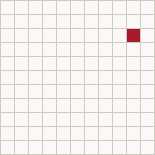
\includegraphics[width=0.22\linewidth]{figures/obs_own_head.png} &
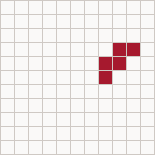
\includegraphics[width=0.22\linewidth]{figures/obs_own_body.png} &
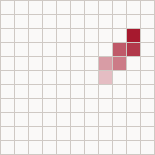
\includegraphics[width=0.22\linewidth]{figures/obs_own_age.png} &
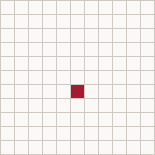
\includegraphics[width=0.22\linewidth]{figures/obs_enemy_heads.png}\\
\footnotesize own head & \footnotesize own body & \footnotesize own age & \footnotesize enemy heads\\[4pt]
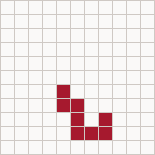
\includegraphics[width=0.22\linewidth]{figures/obs_enemy_bodies.png} &
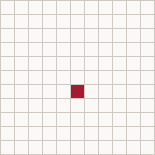
\includegraphics[width=0.22\linewidth]{figures/obs_danger.png} &
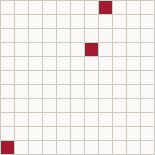
\includegraphics[width=0.22\linewidth]{figures/obs_food.png} &
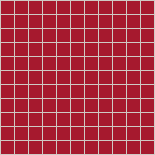
\includegraphics[width=0.22\linewidth]{figures/obs_health.png}\\
\footnotesize enemy bodies & \footnotesize dangerous heads & \footnotesize food & \footnotesize health
\end{tabular}
\captionof{figure}{The eight planes for the orange snake in the duel position of
Figure~\ref{fig:duel-board}. Shade is the plane's value: the age plane fades from head to
tail, and the health plane is uniform.}
\label{fig:obs-planes}
\end{center}

\begin{keybox}[Egocentric, not hand-engineered]
Every plane is a direct transcription of the board; nothing is computed that the rules do
not already state. The legacy agent's A* path quality and dead-end lookahead are gone.
Three design choices still matter:
\begin{itemize}
\item \textbf{Self versus others} rather than ``snake 0 versus snake 1''. Swapping two
  snakes swaps their observations, which is tested, so one network can play any seat.
\item \textbf{The age plane} tells the network which segment leaves next, which is how
  it can know a tail cell will be free.
\item \textbf{The dangerous-heads plane} restates the head-to-head rule
  (Chapter~\ref{ch:game}) in a form a convolution can read locally.
\end{itemize}
\end{keybox}

\begin{warnbox}[Segments that share a cell]
At the start all three segments of a snake share one cell, and after eating the tail is
duplicated. Planes are written tail-first, so where segments overlap the one nearest the
head wins. The duplicated tail cell therefore reads $2/L$ rather than $1/L$ on the
turn after eating, a deliberate and documented simplification.
\end{warnbox}

\section{Walls}

Nothing in the eight planes marks the edge of the board. The network supplies it itself:
it appends a constant plane of ones before the first convolution. Zero padding then
makes that plane drop to $0$ exactly outside the board, so every filter that touches the
edge can tell. This avoids an extra input plane that would be identical in every
position.

\section{The arena window}\label{sec:window}

A network whose first fully connected layer expects $64\cdot 11\cdot 11$ inputs is
bound to an $11\times11$ board. The arena network instead reads a fixed-size window
around its own head.

\begin{defbox}[Window observation]
For odd $W$ and viewer $k$ with head at $(r_0,c_0)$, the window observation is
$w^k\in[0,1]^{9\times W\times W}$ with
\[
  w^k_{c}(i,j) =
  \begin{cases}
    o^k_c\bigl(r_0 - \lfloor W/2\rfloor + i,\ c_0 - \lfloor W/2\rfloor + j\bigr)
      & \text{if that cell is on the board,}\\
    0 & \text{otherwise,}
  \end{cases}
\]
for the eight planes $c=0,\dots,7$, plus a ninth \emph{wall} plane equal to $1$ exactly
where the window extends past the board. The arena uses $W=17$ on a $19\times19$ board.
\end{defbox}

\begin{center}
\setlength{\tabcolsep}{6pt}
\begin{tabular}{@{}ccc@{}}
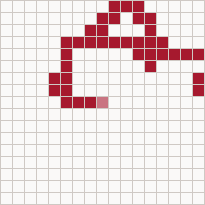
\includegraphics[width=0.27\linewidth]{figures/window_bodies.png} &
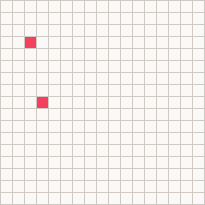
\includegraphics[width=0.27\linewidth]{figures/window_food.png} &
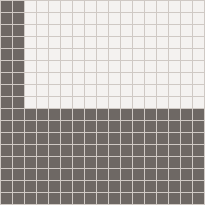
\includegraphics[width=0.27\linewidth]{figures/window_wall.png}\\
\footnotesize snakes (heads lighter) & \footnotesize food & \footnotesize wall plane
\end{tabular}
\captionof{figure}{The $17\times17$ window of one arena snake at turn 120, centred on its
head. The grey wall plane marks the part of the window that hangs off the board.}
\label{fig:window}
\end{center}

Because the window always sits on the snake's own head, its centre is always ``me''. The
same weights serve any board size and any number of opponents. The crop is fully
vectorised: row and column index grids are built from the head positions, clipped to the
board for the lookup, and multiplied by an in-bounds mask.

\section{Rewards}

\begin{defbox}[Reward functions]
\textbf{\code{winloss}} (default for $S>1$): $+1$ to the winner when the game ends,
$-1$ to a snake on the turn it dies, and $0$ to snakes that die together on the final
turn of a game with no winner.

\textbf{\code{food}} (default for $S=1$): $+1$ per food eaten, $-1$ on death.

\textbf{Training reward}: \code{winloss} plus a small shaping term,
\[
  r_t^k = R^k_t + 0.05\cdot\mathbf{1}[\,k \text{ ate at } t\,].
\]
\end{defbox}

The shaping bonus is twenty times smaller than a win, small enough that the agent never
prefers eating to winning. It is large enough to make early exploration find food before
it can find wins.

\section{Episode boundaries and padding}

With two snakes, a death ends the game. With six it does not, and a dead snake's seat
keeps producing ``transitions'' until the game ends. These are padding: its actions are
ignored and its rewards are zero.

\begin{defbox}[Dones and the active mask]
\[
  \text{done}^k_t = \text{died}^k_t \;\vee\; \text{game\_over}_t,
  \qquad
  \text{active}^k_t = \text{alive}^k_{t-1}\wedge \neg\,\text{over}_{t-1}.
\]
Every slot of a game that ends receives \emph{done}, so no slot's trajectory runs into the
next game. A transition is real only where \emph{active} holds, and the trainer masks
everything else out of the loss.
\end{defbox}

\begin{warnbox}[Found in review]
An earlier version set \emph{done} only for snakes alive at the end, so with three or more
snakes a dead seat never saw an episode boundary, and nothing marked its padding steps.
A probe of 64 games with 3 snakes over 400 turns counted 12{,}682 such zombie
transitions. Two-snake games were never affected, but the arena would have been. The
fix above landed before any multi-snake training.
\end{warnbox}

\section{The action mask}

\begin{defbox}[Action mask]
Let the \emph{blocked} cells be every segment of every living snake except its last,
since tails move away. Move $a$ is \emph{safe} for snake $k$ if
$x^k_0+\delta(a)$ is on the board and not blocked. A duplicated tail stays blocked
automatically, because its copy is the second-to-last segment.
\end{defbox}

The policy's logits for unsafe moves are set to $-10^9$ before the softmax, so the network
never wastes probability, or gradient, on walking into a wall. If no move is safe, all
four are allowed and the snake dies anyway. The mask is deliberately optimistic in two
ways that the network must learn to handle itself:
\begin{itemize}
\item it assumes enemy tails move, so it cannot know that an enemy is about to eat and
  keep its tail where it is;
\item it ignores head-to-head risk, which the dangerous-heads plane exposes instead.
\end{itemize}

\chapter{Scripted Opponents and Measurement}\label{ch:baselines}

Self-play has no fixed point of reference: the opponent improves as fast as the
learner. To know whether the learner is actually getting better, it is scored against
opponents that never change. This chapter introduces five hand-written bots, ranks them
against each other, and describes the harness that turns matches into numbers with error
bars.

\section{Five bots}

Every bot, and every learned agent, has the same interface: a function from a batched
game state and a seat index to one action per game. The harness cannot tell them apart.

\begin{defbox}[The baseline bots]
\begin{description}[leftmargin=1.2em,font=\normalfont\bfseries\color{inkblue}]
\item[random] Uniform over the four moves, fatal ones included.
\item[safe\_random] Uniform over the moves the action mask allows.
\item[greedy] Among safe moves, the one that most reduces the Manhattan distance to the
  nearest food.
\item[flood\_fill] The strongest bot, built as a Battlesnake heuristic should be. See
  below.
\item[hamiltonian] For a single snake on an even board: follow a fixed cycle through
  every cell. It never collides and eventually fills the board.
\end{description}
\end{defbox}

\begin{algbox}[Flood-fill bot, per game]
\begin{enumerate}
\item Start from the safe moves.
\item \textbf{Avoid losing head-to-heads.} Drop moves into a cell that an enemy at least
  as long could also enter next turn, unless that leaves nothing.
\item \textbf{Keep room to move.} Label the connected free regions of the board (tails
  count as free) with \code{scipy.ndimage.label}. Keep moves whose region has at least as
  many cells as the snake is long; if none do, keep those with the largest region.
\item \textbf{Eat when it matters.} The snake is \emph{hungry} if its health is $\le 30$ or
  any enemy is at least as long. Hungry: choose by nearest food, then larger region.
  Otherwise: choose by larger region, then nearest food.
\item Break remaining ties at random.
\end{enumerate}
\end{algbox}

\section{The baseline ladder}

Each pair of adjacent bots played 500 games on $11\times11$.

\begin{center}
\begin{tabular}{@{}lcccc@{}}
\toprule
\textbf{Matchup} & \textbf{Wins} & \textbf{Draws} & \textbf{Losses} & \textbf{Win rate (95\% CI)}\\
\midrule
flood\_fill \emph{vs} greedy & 370 & 22 & 108 & 74.0\% \ (70.0--77.7)\\
greedy \emph{vs} safe\_random & 401 & 6 & 93 & 80.2\% \ (76.5--83.5)\\
safe\_random \emph{vs} random & 498 & 1 & 1 & 99.6\% \ (98.6--99.9)\\
\bottomrule
\end{tabular}
\end{center}

The ordering random $<$ safe\_random $<$ greedy $<$ flood\_fill is strict and wide, and is
enforced by a test that requires every step of the ladder to exceed 60\%.

\begin{keybox}[What the ladder says about the game]
Greedy is a strong-looking strategy: it grows quickly and wins most head-to-heads
because it is usually longer. Flood-fill still beats it three games in four, almost
entirely by not trapping itself. Space, not food, is the scarce resource on an
$11\times11$ board with two snakes on it. The learned agent rediscovers this
(Chapter~\ref{ch:duel}).
\end{keybox}

\subsection{Single-snake references}

On its own, the greedy bot scores a mean of 23.7 food per game (95\% CI 22.9--24.5;
max 57) over 500 games on $11\times11$ before it traps itself. The Hamiltonian bot is the
opposite extreme: on $8\times8$ with $h_{\max}=64$, it fills the entire board in every one of
20 games, finishing at length $65$ (Chapter~\ref{ch:game}) with a score of $62$.

\section{The evaluation harness}

\begin{algbox}[\code{run\_matches(policies, n\_games, seed)}]
\begin{enumerate}
\item Create one environment per game, $N = n_{\text{games}}$, with policy $i$ in seat $i$.
\item Step all games together; every policy acts for its seat in every game.
\item Record each environment's \emph{first} finished game only. Later games in an
  environment that auto-reset are ignored, so short games are not over-counted.
\item Per seat: a \emph{win} if it is the winner; a \emph{draw} if there is no winner and
  the seat was active on the final turn; otherwise a \emph{loss}.
\end{enumerate}
\end{algbox}

\begin{warnbox}[Counting each game exactly once]
Without step 3, a fast-finishing environment would contribute several games while a slow
one contributed one, biasing results toward whatever ends games quickly. A deterministic
test pins this down. Two snakes that only ever move up die at the top wall at turn
$r_0+1$, where $r_0$ is their start row. Every win, draw and loss, and the mean game
length, is therefore predictable from the start rows, and the test checks them exactly.
\end{warnbox}

\subsection{Confidence intervals}

\begin{defbox}[Wilson score interval]
For $w$ wins in $n$ games, $\hat p = w/n$ and $z = 1.96$:
\[
  \frac{\hat p + \frac{z^2}{2n} \;\pm\; z\sqrt{\frac{\hat p(1-\hat p)}{n} + \frac{z^2}{4n^2}}}
       {1 + \frac{z^2}{n}} .
\]
\end{defbox}

The Wilson interval behaves well near $0$ and $1$, where most of the interesting results
in this report sit; the naive normal interval would extend past $100\%$ there. For
single-snake scores, a 95\% percentile bootstrap over 2{,}000 resamples gives the interval
on the mean. Every run is reproducible from one seed: environments, food and bots all
draw from seeded generators.

\chapter{Learning by Self-Play}\label{ch:learn}

Both networks are trained with Proximal Policy Optimization (PPO), an on-policy
actor--critic method, in a self-play loop: the policy being trained controls most of the
snakes in every game. This chapter states the objective, the self-play scheme, the
network, and the compute.

\section{Actor and critic}

A single network with parameters $\theta$ has two heads. Given observation $o$, it outputs
action logits, from which a masked softmax gives the policy $\pi_\theta(a\mid o)$, and a
scalar value estimate $V_\theta(o)$ of the return. The value head is what the web page
displays as the network's ``confidence'' (Chapter~\ref{ch:browser}).

\section{Advantages}

\begin{defbox}[Generalized advantage estimation]
For one seat's trajectory with rewards $r_t$ and episode boundaries $d_t$, define the TD
residual and the advantage estimate
\[
  \delta_t = r_t + \gamma\,(1-d_t)\,V(o_{t+1}) - V(o_t),
  \qquad
  \hat A_t = \sum_{l\ge 0} (\gamma\lambda)^l \prod_{m=0}^{l-1}(1-d_{t+m})\;\delta_{t+l},
\]
with $\gamma=0.99$ and $\lambda=0.95$, computed by one backward pass over the rollout. The
value targets are $\hat R_t = \hat A_t + V(o_t)$. The last step of a rollout bootstraps
from the value of the following observation.
\end{defbox}

The factor $(1-d_t)$ is where the dones of Chapter~\ref{ch:obs} matter: since every slot of
a finished game is marked done, no advantage ever leaks from one game into the next game
played in the same environment slot.

\section{The PPO objective}

Let $\pi_{\text{old}}$ be the policy that collected the rollout and
\[
  \rho_t(\theta) = \frac{\pi_\theta(a_t\mid o_t)}{\pi_{\text{old}}(a_t\mid o_t)}.
\]

\begin{defbox}[Clipped surrogate and total loss]
\[
  L^{\text{CLIP}}(\theta) = \E_t\!\left[\min\!\Bigl(\rho_t(\theta)\,\hat A_t,\;
     \clip\bigl(\rho_t(\theta),\,1-\epsilon,\,1+\epsilon\bigr)\,\hat A_t\Bigr)\right],
  \qquad \epsilon = 0.2,
\]
\[
  \mathcal{L}(\theta) = -L^{\text{CLIP}}(\theta)
    + c_v\,\E_t\!\left[\tfrac12\bigl(V_\theta(o_t)-\hat R_t\bigr)^2\right]
    - c_e\,\E_t\!\left[\Hent\bigl(\pi_\theta(\cdot\mid o_t)\bigr)\right],
\]
with $c_v=0.5$ and $c_e=0.01$. Advantages are normalised to zero mean and unit variance
over each batch.
\end{defbox}

\begin{keybox}[Why PPO here]
The game is on-policy friendly: experience is cheap (Chapter~\ref{ch:sim}), and the
data distribution shifts every iteration anyway because the opponent \emph{is} the
policy. PPO's clipping keeps each update close to the policy that gathered the data. That
matters doubly in self-play, where a large jump changes both sides of every game at
once.
\end{keybox}

\section{Self-play}

\begin{algbox}[One training iteration]
\begin{enumerate}
\item With probability $0.3$ per environment, the non-learner seats are played by a
  \emph{frozen snapshot}: one set of past weights, drawn uniformly from a pool for this
  iteration. Otherwise the learner plays every seat.
\item Run $T=64$ turns in all environments, sampling actions from the masked policy.
  Store observations (float16), masks, actions, log-probabilities, values and rewards.
\item Mark a transition \emph{valid} if its seat was played by the learner and was active
  (Chapter~\ref{ch:obs}). Compute GAE over the full rollout, then keep valid transitions
  only.
\item Optimise $\mathcal{L}$ for 4 epochs over the valid transitions in minibatches of
  4{,}096, using Adam (learning rate $2.5\times10^{-4}$, $\epsilon=10^{-5}$) and gradient
  norm clipping at $0.5$.
\item Every 10 iterations, add the current weights to the snapshot pool (the most recent
  20 are kept). Every 25--30 iterations, evaluate against the scripted bots and save a
  checkpoint.
\end{enumerate}
\end{algbox}

\begin{keybox}[Two sources of opponents]
Playing the current self is the strongest signal, and every seat yields training data,
so a two-snake game produces two transitions per turn. Playing frozen past selves guards
against \emph{forgetting}: a policy that only ever meets its current self can drift into a
strategy that loses to something it used to beat. Seats a snapshot plays generate no
training data.
\end{keybox}

Each environment re-draws its opponent type whenever its game ends. In the duel run,
$512$ environments $\times$ $64$ turns gives $32{,}768$ game turns per iteration and
about $55{,}000$ valid learner transitions. The arena run uses $256$ environments of six
snakes each.

\section{The network}

\begin{center}
\begin{tikzpicture}[node distance=0.42cm and 0.38cm,
    layer/.style={node box, minimum height=1.25cm, text width=1.55cm},
    hd/.style={node fill, text width=1.25cm}]
  \node[node soft, text width=1.65cm, minimum height=1.25cm] (in) {input\\[1pt]\scriptsize $C{+}1$ planes\\$H\times W$};
  \node[layer, right=of in] (c1) {conv $3{\times}3$\\\scriptsize 32, ReLU};
  \node[layer, right=of c1] (c2) {conv $3{\times}3$\\\scriptsize 64, ReLU};
  \node[layer, right=of c2] (c3) {conv $3{\times}3$\\\scriptsize 64, ReLU};
  \node[layer, right=of c3] (fc) {linear\\\scriptsize $64HW\!\to\!h$, ReLU};
  \node[hd, above right=0.05cm and 0.5cm of fc] (pi) {policy\\\scriptsize 4 logits};
  \node[hd, below right=0.05cm and 0.5cm of fc] (v) {value\\\scriptsize 1 scalar};
  \draw[flow] (in) -- (c1);
  \draw[flow] (c1) -- (c2);
  \draw[flow] (c2) -- (c3);
  \draw[flow] (c3) -- (fc);
  \draw[flow] (fc.east) -- (pi.west);
  \draw[flow] (fc.east) -- (v.west);
\end{tikzpicture}
\captionof{figure}{The actor--critic. All convolutions use padding 1, so spatial size is
preserved; the extra input plane is the constant ones plane that reveals walls through
zero padding.}
\label{fig:net}
\end{center}

\begin{center}
\begin{tabular}{@{}lccc@{}}
\toprule
& \textbf{Input} $C{+}1,\,H{\times}W$ & \textbf{Hidden} $h$ & \textbf{Parameters}\\
\midrule
Duel network & $9,\ 11\times11$ & 256 & 2{,}042{,}053\\
Arena network & $10,\ 17\times17$ (window) & 128 & 2{,}426{,}597\\
\bottomrule
\end{tabular}
\end{center}

Almost all parameters sit in the first linear layer, $64HW\cdot h$, which is why the arena
network halves $h$ to compensate for its larger window. A fully convolutional design
would remove the dependence on $H\times W$ altogether. The window observation achieves
the same independence from board size while keeping this simple architecture.

\section{Compute}

Both networks trained for 2.5 hours on an Apple M3 Max, using PyTorch's Metal (MPS)
backend for the network and the CPU for the simulator.

\begin{center}
\begin{tabular}{@{}lcc@{}}
\toprule
& \textbf{Seconds per iteration} & \textbf{Relative}\\
\midrule
CPU, 12 threads & $\approx 70$ & $1\times$\\
Apple GPU (MPS) & $\approx 5$--$6$ & $\approx 10\times$\\
\bottomrule
\end{tabular}
\end{center}

\begin{warnbox}[The GPU mattered more than expected]
The network is small, so CPU training looked plausible. In practice the PPO update,
four epochs over $\sim55{,}000$ samples through a $2$M-parameter network, dominated each
iteration, and moving it to the GPU was the difference between a 2.5-hour run and a
day-long one. The simulator stayed on the CPU throughout.
\end{warnbox}

\chapter{Results: The Duel}\label{ch:duel}

The duel network plays two-snake Battlesnake on the standard $11\times11$ board. It
trained for 2.5 hours: 1{,}109 iterations, 36.3 million game turns.

\section{Learning curve}

\begin{center}
\begin{tikzpicture}
\begin{axis}[reportaxis, xmin=0, xmax=37, ymin=0, ymax=100,
  xlabel={self-play game turns (millions)}, ylabel={win rate (\%)},
  legend style={at={(0.5,-0.24)},anchor=north,legend columns=2,/tikz/every even column/.append style={column sep=1.2em}}]
\addplot[color=cmured] table[x=steps, y=flood, col sep=comma] {data/duel_eval.csv};
\addlegendentry{vs flood-fill bot}
\addplot[color=inkblue] table[x=steps, y=greedy, col sep=comma] {data/duel_eval.csv};
\addlegendentry{vs greedy bot}
\addplot[color=rulegrey, dashed, line width=0.9pt, forget plot] coordinates {(0,74) (37,74)};
\node[font=\scriptsize\itshape, color=cmudark, anchor=north west] at (axis cs:14,73) {flood-fill vs greedy: 74\%};
\addplot[color=amber, densely dotted, line width=1pt, forget plot] coordinates {(33.59,0) (33.59,100)};
\node[font=\scriptsize\itshape, color=amber!80!black, anchor=east, align=right] at (axis cs:33.2,40) {selected\\checkpoint};
\end{axis}
\end{tikzpicture}
\captionof{figure}{Win rate of the duel network during training, measured every 25
iterations over 200 games against each bot (deterministic play). The grey line is the
flood-fill bot's own win rate against greedy, for scale.}
\label{fig:duel-curve}
\end{center}

The curve has three phases.
\begin{itemize}
\item \textbf{Survival} (0--4M turns). The network first learns not to die. Against the
  greedy bot it starts at 54\% almost immediately, because greedy plays into dead ends
  that a cautious random walker avoids. Against flood-fill it starts at 11\%.
\item \textbf{Competence} (4--10M). The win rate against flood-fill climbs to about
  80\% by 10.6M turns. From 9M turns on, the network beats flood-fill more often than
  flood-fill beats greedy.
\item \textbf{Refinement} (10--36M). Slow gains to around 90\% against both bots, with
  checkpoint-to-checkpoint noise of a few points, about what 200-game evaluations
  produce.
\end{itemize}

\section{Training dynamics}

\begin{center}
\begin{minipage}{0.49\linewidth}
\begin{tikzpicture}
\begin{axis}[reportaxis, width=\linewidth, height=5cm, xmin=0, xmax=37, ymin=0,
  xlabel={turns (millions)}, ylabel={mean game length},
  title={\small\color{cmudark}Self-play game length}]
\addplot[color=cmured] table[x=steps, y=turns, col sep=comma] {data/duel_train.csv};
\end{axis}
\end{tikzpicture}
\end{minipage}\hfill
\begin{minipage}{0.49\linewidth}
\begin{tikzpicture}
\begin{axis}[reportaxis, width=\linewidth, height=5cm, xmin=0, xmax=37, ymin=0, ymax=1.2,
  xlabel={turns (millions)}, ylabel={policy entropy (nats)},
  title={\small\color{cmudark}Policy entropy}]
\addplot[color=inkblue] table[x=steps, y=entropy, col sep=comma] {data/duel_train.csv};
\addplot[color=rulegrey, dashed, line width=0.9pt] coordinates {(0,1.0986) (37,1.0986)};
\node[font=\scriptsize\itshape, color=cmudark, anchor=north east] at (axis cs:36.5,1.07) {uniform over 3 moves, $\ln 3$};
\end{axis}
\end{tikzpicture}
\end{minipage}
\captionof{figure}{Left: mean length of self-play games, which grows from about 30 to
about 185 turns as both sides learn to survive. Right: entropy of the masked policy,
falling from 0.95 nats (close to uniform over the usual three safe moves) to about 0.3
nats as play becomes decisive.}
\label{fig:duel-dynamics}
\end{center}

Self-play games lengthening sixfold is the clearest sign that both copies of the network
are improving together: neither side finds easy kills against itself any more. Entropy
falls steadily but never collapses. The $0.01$ entropy bonus keeps enough randomness
that exploration continues to the end of the run.

\section{Final evaluation}

The checkpoint with the best score (win rate $+\,\tfrac12$ draw rate against flood-fill)
was iteration 1{,}025, at 33.6M turns. It was then evaluated on 1{,}000 \emph{fresh}
games against each bot, with a seed never used during training or selection.

\begin{center}
\begin{tabular}{@{}lcccccc@{}}
\toprule
\textbf{Opponent} & \textbf{W} & \textbf{D} & \textbf{L} & \textbf{Win rate (95\% CI)} &
  \textbf{Game length} & \textbf{Final length}\\
& & & & & \footnotesize turns & \footnotesize net\ /\ bot\\
\midrule
flood\_fill & 914 & 4 & 82 & \textbf{91.4\%} \ (89.5--93.0) & 99.3 & 13.1 / 12.5\\
greedy & 902 & 64 & 34 & \textbf{90.2\%} \ (88.2--91.9) & 63.1 & \hphantom{1}9.4 / 10.5\\
safe\_random & 994 & 2 & 4 & \textbf{99.4\%} \ (98.7--99.7) & 36.7 & \hphantom{1}8.3 / \hphantom{1}4.0\\
\bottomrule
\end{tabular}
\end{center}

\begin{keybox}[It wins without out-eating its opponent]
Against the greedy bot the network wins 90\% of games while ending them \emph{shorter}
than its opponent, at 9.4 segments against 10.5. It is not winning the race for food. It
wins by position: cutting off space, steering the opponent toward walls and its own
body, and declining head-to-heads it would lose. These are exactly the ideas built into
the flood-fill bot by hand, and that bot also beats greedy. The network found them from a
$\pm1$ signal, and against flood-fill itself it wins 91\% of games.
\end{keybox}

\begin{warnbox}[Draws against greedy]
6.4\% of games against greedy are draws, against 0.4\% for flood-fill. Greedy charges
straight at food; when both snakes are equally long and arrive at the same cell, both
die. The network does not always avoid this; it treats a draw as better than the
risk of losing. A reward that penalised draws more than $0$ would push it further.
\end{warnbox}

\chapter{Results: The Arena}\label{ch:arena}

\begin{center}
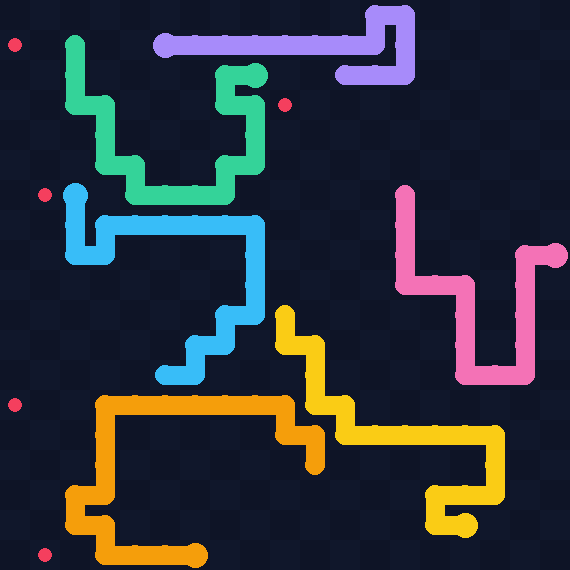
\includegraphics[width=0.56\linewidth]{figures/arena_board.png}
\captionof{figure}{An arena game at turn 120: six copies of the arena network on a
$19\times19$ board, all six still alive.}
\label{fig:arena-board}
\end{center}

The arena is a free-for-all: six snakes on a $19\times19$ board, with at least six food
on the board at all times, so a crowded board does not simply starve. The arena network
reads the $17\times17$ window of Section~\ref{sec:window}, so the same weights also play
the browser's arena with anywhere from 2 to 8 snakes.

\section{Measuring a six-player game}

\begin{keybox}[One against five]
A six-player game cannot be scored as a single head-to-head. Instead the network takes
one seat and the other \emph{five} are all the same scripted bot. If the network were
exactly as good as the bot, it would win $1/6\approx16.7\%$ of games. Every arena win rate
should be read against that fair share, not against 50\%.
\end{keybox}

\section{Learning curve}

\begin{center}
\begin{tikzpicture}
\begin{axis}[reportaxis, xmin=0, xmax=16.5, ymin=0, ymax=100,
  xlabel={self-play game turns (millions)}, ylabel={win rate as 1 of 6 snakes (\%)},
  legend style={at={(0.5,-0.24)},anchor=north,legend columns=2,/tikz/every even column/.append style={column sep=1.2em}}]
\addplot[color=cmured] table[x=steps, y=flood, col sep=comma] {data/arena_eval.csv};
\addlegendentry{vs $5\times$ flood-fill}
\addplot[color=inkblue] table[x=steps, y=greedy, col sep=comma] {data/arena_eval.csv};
\addlegendentry{vs $5\times$ greedy}
\addplot[color=rulegrey, dashed, line width=0.9pt, forget plot] coordinates {(0,16.67) (16.5,16.67)};
\node[font=\scriptsize\itshape, color=cmudark, anchor=north east] at (axis cs:16.2,15.5) {fair share, $1/6$};
\addplot[color=amber, densely dotted, line width=1pt, forget plot] coordinates {(8.847,0) (8.847,100)};
\node[font=\scriptsize\itshape, color=amber!80!black, anchor=north west, align=left] at (axis cs:9.0,30) {highest\\60-game score};
\end{axis}
\end{tikzpicture}
\captionof{figure}{Arena win rate during training, evaluated every 30 iterations over 60
games. The dotted line marks the checkpoint that scored highest on these small
evaluations; it was not the one finally used (see below).}
\label{fig:arena-curve}
\end{center}

Against five greedy bots the network is ahead of its fair share from the very first
checkpoint, at 77\% after half a million turns. Greedy bots in a crowd mostly kill each
other, and a snake that merely avoids them survives. Against five flood-fill bots it
starts below fair share, at 8\%, and passes 40\% within 4M turns.

\begin{center}
\begin{tikzpicture}
\begin{axis}[reportaxis, height=4.8cm, xmin=0, xmax=16.5, ymin=0,
  xlabel={self-play game turns (millions)}, ylabel={mean game length}]
\addplot[color=cmured] table[x=steps, y=turns, col sep=comma] {data/arena_train.csv};
\end{axis}
\end{tikzpicture}
\captionof{figure}{Mean length of six-snake self-play games, growing from about 50 turns
to over 1{,}000 as the snakes learn to share the board without colliding.}
\label{fig:arena-length}
\end{center}

\section{Choosing the checkpoint}

\begin{warnbox}[The ``best'' checkpoint was not the best]
Checkpoints were scored during training on only 60 games each. Picking the maximum of 33
noisy scores favours a checkpoint that got lucky, a selection bias. The highest scorer
was iteration 540, at 8.8M turns, yet later checkpoints looked at least as strong. Two
candidates were therefore compared on a separate seed, 777, never used for the final
numbers:
\begin{center}
\begin{tabular}{@{}lcc@{}}
\toprule
\textbf{200 games, seed 777} & \textbf{vs $5\times$ flood-fill} & \textbf{vs $5\times$ greedy}\\
\midrule
iteration 540 (highest 60-game score) & 35.0\% & 81.0\%\\
iteration 971 (end of training) & \textbf{47.5\%} & \textbf{92.5\%}\\
\bottomrule
\end{tabular}
\end{center}
The final checkpoint was chosen. The reported results below come from a third seed,
12345, so neither the training-time scores nor this comparison inflates them.
\end{warnbox}

\section{Final evaluation}

\begin{center}
\begin{tabular}{@{}lcccccc@{}}
\toprule
\textbf{Opponents} & \textbf{W} & \textbf{D} & \textbf{L} & \textbf{Win rate (95\% CI)} &
  \textbf{Game length} & \textbf{Final length}\\
\textbf{($\times5$)} & & & & & \footnotesize turns & \footnotesize net\ /\ bots\\
\midrule
flood\_fill & 134 & 2 & 164 & \textbf{44.7\%} \ (39.1--50.3) & 385.2 & 43.0 / 25.1\\
greedy & 264 & 2 & 34 & \textbf{88.0\%} \ (83.8--91.2) & 163.8 & 24.7 / 14.3\\
safe\_random & 296 & 0 & 4 & \textbf{98.7\%} \ (96.6--99.5) & 205.7 & 32.4 / \hphantom{1}5.3\\
\bottomrule
\end{tabular}
\end{center}
\begin{center}
\footnotesize\color{cmudark} 300 games per row; fair share $16.7\%$.
\end{center}

\begin{keybox}[Nearly three times its fair share]
Against a table of five flood-fill bots, each built to protect its own space, the network
wins 44.7\% of six-player games, $2.7\times$ the $16.7\%$ an equal player would get. It
also grows much longer than its opponents, 43 segments against 25. In a crowded game,
length is both a weapon (it wins head-to-heads) and a wall that takes space from
everyone else, and the network uses it as both.
\end{keybox}

\section{The window generalises}

Because the network never sees the whole board, nothing in it depends on the board size
or the number of snakes. In the browser it plays two to eight snakes on $19\times19$
without retraining. No numbers are reported for configurations other than the
six-snake training setup, so how well this generalisation holds up is unmeasured.

\chapter{Into the Browser}\label{ch:browser}

The final layer puts both networks on a static web page. There is no server: the game
rules, the networks and the rendering all run in the visitor's browser.

\section{Architecture}

\begin{center}
\begin{tikzpicture}[node distance=0.7cm and 1.1cm]
  \node[node soft, text width=2.4cm] (ckpt) {PyTorch\\checkpoint};
  \node[node box, right=of ckpt, text width=2.4cm] (onnx) {ONNX graph\\\footnotesize opset 17};
  \node[node fill, right=of onnx, text width=2.6cm] (ort) {ONNX Runtime Web\\\footnotesize WebAssembly};
  \node[node box, below=0.9cm of ort, text width=3.0cm] (rules) {\code{rules.js}\\\footnotesize rules, observations};
  \node[node box, left=of rules, text width=2.9cm] (loop) {\code{app.js}\\\footnotesize clock, input, panel};
  \node[node soft, left=of loop, text width=2.4cm] (canvas) {Canvas\\\footnotesize 60 frames/s};
  \draw[flow] (ckpt) -- node[lbl,above=1pt]{export} (onnx);
  \draw[flow] (onnx) -- (ort);
  \draw[flow] (rules) -- node[lbl,right]{observations} (ort);
  \draw[flow] (ort.south west) to[bend right=15] node[lbl,above left,pos=0.4]{moves} (loop.north east);
  \draw[flow] (loop) -- (rules);
  \draw[flow] (loop) -- (canvas);
\end{tikzpicture}
\end{center}

\begin{itemize}
\item \textbf{Export.} Each checkpoint is exported to ONNX (opset 17) with a dynamic batch
  dimension. ONNX Runtime then runs the export on random inputs, and the export
  script requires its logits and values to match PyTorch to within a relative $10^{-3}$.
\item \textbf{Inference.} ONNX Runtime Web 1.20.1 runs on WebAssembly with a single
  thread, which avoids the cross-origin isolation headers that multi-threading would
  require of the host. The duel network (8.2\,MB) loads with the page; the arena network
  (9.7\,MB) loads the first time Arena mode is opened.
\item \textbf{Rules.} \code{rules.js} is a single-game port of the engine, including the
  eight-plane and window observations, and is checked against the Python engine on
  6{,}400 transitions (Chapter~\ref{ch:verify}). What the page shows is the game the
  networks were trained on, not an approximation of it.
\end{itemize}

\section{Modes}

\begin{center}
\begin{tabular}{@{}llp{0.5\linewidth}@{}}
\toprule
\textbf{Mode} & \textbf{Board} & \textbf{Seats}\\
\midrule
AI vs AI & $11\times11$ & duel network in both seats, sampling from its policy\\
You vs AI & $11\times11$ & duel network (most likely move) against the player\\
AI vs bot & $11\times11$ & duel network against the greedy bot\\
Arena & $19\times19$ & 2--8 copies of the arena network, sampling; $f_{\min}$ equals the snake count\\
\bottomrule
\end{tabular}
\end{center}

\begin{warnbox}[Two deterministic copies mirror each other]
With both seats playing their most likely move, the first AI-vs-AI games ended in
identical head-on draws on turn four. The starts are symmetric, so two copies of one
deterministic policy make symmetric choices into the centre food. The all-AI modes
therefore \emph{sample} from the policy, as in training. The modes against a human or a
bot play the most likely move, as in evaluation.
\end{warnbox}

A side panel shows, live, the move probabilities of one network for its next turn and
its value estimate $V_\theta$, together with each snake's length and health.

\section{Continuous motion from a turn-based game}

The game advances in whole turns, but the page must look fluid, like a modern Snake
game. The fix is to separate logic from drawing: the rules move in discrete steps, and
the renderer interpolates between the last two states.

\begin{defbox}[Interpolated body]
Let $p_0,\dots,p_{L'-1}$ be a snake's cells before the latest turn and $c_0,\dots,c_{L-1}$
after it, so $c_i=p_{i-1}$ for $i\ge1$. At fraction $t\in[0,1]$ of the turn, the snake is
drawn as the polyline
\[
  \bigl(\,(1-t)\,p_0 + t\,c_0,\;\; c_1,\;\dots,\;c_{L-1},\;\; (1-t)\,p_{L'-1} + t\,c_{L-1}\,\bigr)
\]
through cell centres, stroked with round joins and caps.
\end{defbox}

At $t=1$ the head sits at $c_0$ and the tail at $c_{L-1}$. At the start of the next turn,
$t=0$, they sit at $p'_0 = c_0$ and $p'_{L-1}=c_{L-1}$: the drawing is continuous across
turn boundaries. When a snake has just eaten, the duplicated tail makes the last two
points coincide, so the tail correctly stays put.

\begin{warnbox}[Three bugs on the way to fluid]
\begin{enumerate}
\item \textbf{Ease-in, ease-out.} The first version eased each step with a smoothstep
  curve. Its velocity is zero at both ends of every turn, so the snake visibly stopped at
  every cell. Linear interpolation moves at constant speed.
\item \textbf{Stalls between turns.} Each turn waited for the network's next move before
  starting. The fix computes the AI's moves for the next turn while the current one
  animates, and drives the game from the animation loop on a fixed-cadence clock. A
  frame-by-frame measurement then showed the snake moving in every one of 90 consecutive
  frames.
\item \textbf{Diagonal tails.} The first polyline joined the moving tail straight to
  $c_{L-2}$, skipping $c_{L-1}$, the cell the tail is entering. At a corner that cut the
  corner diagonally. Including $c_{L-1}$, as in the definition above, keeps every segment
  on the grid.
\end{enumerate}
\end{warnbox}

Player input is buffered and read at the last moment before each turn. Arrow keys, WASD,
swipes, and clicks on the board, which steer toward the clicked cell, all feed the same
queue. A reversal onto the snake's own neck is ignored rather than allowed to kill it.

\chapter{Limitations and Next Steps}\label{ch:limits}

\section{What the results do not show}

\begin{warnbox}[Caveats on the numbers]
\begin{itemize}
\item \textbf{One seed per network.} Each network is a single 2.5-hour run. The
  confidence intervals cover evaluation noise, not training noise. A second seed could
  land a few points higher or lower.
\item \textbf{Scripted opponents only.} The win rates are against hand-written bots.
  They establish that the networks are strong relative to sensible heuristics, not how
  they rank among competitive Battlesnake agents or human players.
\item \textbf{Exact replay needs more care.} The simulator and evaluation are seeded and
  reproducible. Training on the Apple GPU is not bit-for-bit deterministic, so rerunning
  training reproduces the curves only statistically.
\item \textbf{Arena generalisation is unmeasured.} The arena network is evaluated only
  in its training configuration of six snakes. Its play with 2, 3 or 8 snakes in the
  browser is plausible but untested.
\item \textbf{Draws are free.} The reward gives a draw $0$, the same as a game still in
  progress. Against greedy this leaves 6.4\% of games drawn (Chapter~\ref{ch:duel}).
\end{itemize}
\end{warnbox}

\section{Next steps}

\begin{keybox}[An algorithm comparison]
The environment and harness were built so that algorithms can be compared fairly, and
this is the natural next experiment. DQN and its Rainbow components (double Q-learning,
dueling heads, prioritised replay, $n$-step returns), A2C and PPO would each be trained
on the same task with the same budget of environment turns, across several seeds,
and compared on learning curves and final win rates. Value-based methods face a
particular challenge in self-play, where the replay buffer holds games against
opponents who no longer exist.
\end{keybox}

\begin{itemize}
\item \textbf{A league and Elo ratings.} Rate every checkpoint against every other, so
  progress is measured within self-play itself and not only against fixed bots.
\item \textbf{A fully convolutional network.} Removing the large linear layer would make
  the duel network board-size independent too, and cut its size several-fold.
\item \textbf{A public ladder.} The rules follow the official game, so the duel network
  could play live on the public Battlesnake arena behind a small server.
\item \textbf{Reward design.} Penalise draws, or rank the five losers in the arena by
  survival time, so that coming second is worth more than coming last.
\end{itemize}


\appendix
\chapter{Hyperparameters}\label{app:hparams}

\begin{center}
\begin{tabular}{@{}lll@{}}
\toprule
\textbf{Setting} & \textbf{Duel} & \textbf{Arena}\\
\midrule
Board, snakes & $11\times11$, 2 & $19\times19$, 6\\
Minimum food $f_{\min}$ & 1 & 6\\
Observation & full board, 8 planes & $17\times17$ window, 9 planes\\
Hidden width $h$ & 256 & 128\\
Parallel games $N$ & 512 & 256\\
Rollout length $T$ & 64 & 64\\
Discount $\gamma$, GAE $\lambda$ & 0.99, 0.95 & 0.99, 0.95\\
Clip $\epsilon$ & 0.2 & 0.2\\
Epochs, minibatch & 4, 4{,}096 & 4, 4{,}096\\
Optimiser & Adam, $2.5\times10^{-4}$, $\epsilon{=}10^{-5}$ & same\\
Value coef.\ $c_v$, entropy coef.\ $c_e$ & 0.5, 0.01 & 0.5, 0.01\\
Gradient-norm clip & 0.5 & 0.5\\
Food bonus & 0.05 & 0.05\\
Snapshot opponent probability & 0.3 & 0.3\\
Snapshot pool size, interval & 20, every 10 iterations & 20, every 10 iterations\\
Evaluation & every 25 its., 200 games & every 30 its., 60 games\\
Wall-clock budget & 2.5\,h & 2.5\,h\\
Iterations, game turns & 1{,}109, 36.3M & 971, 15.9M\\
Reported checkpoint & iteration 1{,}025 & iteration 971\\
\bottomrule
\end{tabular}
\end{center}

\chapter{Reproducing the Results}\label{app:repro}

Everything runs through \code{uv}. The training extras (PyTorch, ONNX, Pillow) are an
optional dependency group.

\begin{lstlisting}[language=bash]
uv run pytest                                  # 106 tests
uv run python scripts/benchmark_env.py         # simulator throughput
uv run python scripts/evaluate.py flood_fill greedy --games 500

uv sync --group train
# duel network
uv run --group train python scripts/train_selfplay.py --device mps --hours 2.5
uv run --group train python scripts/final_eval.py runs/selfplay/best.pt --games 1000
# arena network
uv run --group train python scripts/train_selfplay.py --run-dir runs/arena \
    --board 19 --num-snakes 6 --window 17 --min-food 6 --hidden 128 \
    --num-envs 256 --device mps --hours 2.5
uv run --group train python scripts/final_eval.py runs/arena/latest.pt \
    --board 19 --num-snakes 6 --min-food 6 --games 300 --out results/ppo_arena.json
# browser assets, then serve the demo
uv run --group train python scripts/build_web_assets.py --run-dir runs/selfplay \
    --final-eval results/ppo_selfplay.summary.json
python3 -m http.server --directory web 8000
# this report's figures
uv run --group train python docs/report/make_figures.py
\end{lstlisting}

All evaluation numbers in this report are stored as JSON in \code{results/}, alongside
the full per-iteration training logs and configurations of both runs.

\chapter{Repository Map}\label{app:repo}

\begin{center}
\begin{tabular}{@{}lp{0.62\linewidth}@{}}
\toprule
\textbf{Path} & \textbf{Contents}\\
\midrule
\code{snake\_rl/env/} & rules, observations, rewards, batched \code{SnakeEnv}, terminal renderer\\
\code{snake\_rl/baselines/} & random, safe\_random, greedy, flood\_fill and hamiltonian bots\\
\code{snake\_rl/agents/} & actor--critic network and its harness wrapper\\
\code{snake\_rl/eval/} & match runner with Wilson and bootstrap intervals\\
\code{scripts/} & training, evaluation, export, benchmarking, play, GIF rendering\\
\code{tests/} & the 106-test suite, including the reference oracle\\
\code{web/} & the browser demo: rules port, app, models\\
\code{results/} & evaluation JSON and training logs\\
\code{docs/report/} & this report and the script that draws its figures\\
\bottomrule
\end{tabular}
\end{center}


\end{document}
